% !TEX TS-program = xelatex
% !TEX encoding = UTF-8 Unicode

\providecommand{\home}{../..}
\documentclass[\home/main.tex]{subfiles}

\begin{document}

\chapter{Towards learning robotic manipulation of clothing} \label{ch:towards_robotic_folding}
\todo{kan je hier nog iets meer naar je eigen werk refereren? dataset paper, instrumentatie paper.}
\todo{figuren toevoegen: ons werk vs ander werk. Bv fiducial marker cloth en onze instrumented cloth.}
In this dissertation, we considered the problem of learning robotic folding of clothing items by using simulation, smart clothing and learning task progression from human demonstrations. In this chapter, we zoom out to take a birds-eye perspective on the field of robotic cloth folding in order to highlight future areas of improvement. Our goal is to describe high-potential areas of research that, according to the research done in this dissertation, require further investigation for the field to advance towards learning robotic manipulation of clothing articles.

\section{Improving sample efficiency}

Data-driven approaches have triggered new developments for solving robotic manipulation problems. In the context of robotic cloth folding, we believe data-driven robotic perception and control will remain omnipresent to learn cloth dynamics, material properties and sensorimotor skills by interacting with the environment. In order to capitalize on learning-based methods, future research has to focus on improving the sample efficiency of these data-hungry methods. This need is imperative for the robotics domain where experimentation with real robots is expensive. 

\subsection{Decouple end-to-end learning}
End-to-end learning offers optimization in unstructured environments with system imperfections by viewing the system holistically. However, it can lead to an immoderate amount of required training data. Hence, a first evident way to reduce data requirements is decoupling end-to-end learning into pipelines with dedicated modules. 
% Decouple e2e: learn submodules
We have demonstrated deconstructing end-to-end learning in \cref{ch:instrumentation} where we used a smart cloth that autonomously communicates its state. This is in stark contrast to current research that engineers vision pipelines \autocite{Wu2020} which potentially fails outside laboratory environments or incorporate learning the state implicitly in the model \autocite{Matas2018}. 
Another instance of decoupling the pipeline can be done by learning as much as possible offline. Batch reinforcement learning, which was introduced in \cref{subsec:lit_rl}, aims to maximally distil the knowledge in a static dataset. Theoretically, this is what Q-learning achieves: learn an optimal policy with suboptimal demonstrations \autocite{Sutton2018}. However, the deep variants have shown to be susceptible to performance collapse when only off-policy data is used \autocite{hausknecht2016policy}. Current research in batch RL is ongoing and merits high potential for reducing the amount of data required for learning. Using batch RL is also a way to commit to the appeal to make learning look as much as possible as supervised learning. Indeed, the same way that supervised learning has turned data into strong pattern recognizers, batch RL can turn data into strong decision-making engines. 
A final implementation of learning offline is shown in this research (\cref{ch:reward_functions}), where we learned a semantic meaningful representation for the task using demonstrations. By generating pseudotasks, the agent can self-supervise its own learning process and acquire task-relevant representations without requiring real robot time. We elaborate on learning and using representations in \cref{sec:towards_sensing_representation}. 

% Decouple e2e: do not learn all submodules
Ultimately, \emph{not every part of the pipeline has to be learned}.
The data requirement of learned systems can be circumvented by incorporating available prior knowledge about the task. The body of knowledge described in \cref{sec:lit_cloth_folding_pipelines} can be used as a prior for learning. For example, when learning from interaction to achieve wrinkle-free folding, the canonical way of defining the reward is a sparse signal indicating whether the cloth is folded or not. However, when end-to-end learning was not prevalent in the robotics folding community, researchers exploited gravity as a way to unfold clothing and remove wrinkles \autocite{Doumanoglou2016,Maitin2010}. This prior knowledge of exploiting gravity can be structured into the reward or task by driving the agent towards lifting the piece of cloth in the air.
Besides incorporating task knowledge, analytical models can improve learning time. For example, the work of \textcite{Zhang2015} and our work in \cref{ch:sim} define the action space in joint space, with each action being a movement of one joint with a fixed delta angle in each direction or remain stationary. However, in both cases the inverse kinematics of the robot is known which implies that the action space could be defined as delta movements of the end-effector in Cartesian space. In the case of a 7 \gls{DOF} arm, this example reduces the options in action space from 21 options (7 joints each having 3 options) to 6 options (forward, up, right and the reverse options). Additionally, the robot does not require learning inverse kinematics when it is already solved by an external module. However, this example would be difficult to realize in case the kinematics are ill-defined, for example, when the robot arm contains a large degree of kinematic redundancy. 

\subsection{Curriculum learning}
A second approach for improving sample efficiency is adjusting the task instantiation to the skills already acquired by the agent. This principle of gradually ramping up the task difficulty is known as \emph{curriculum learning} \autocite{Selfridge1985}. Different methods exist for introducing curricula. In robotic folding, it is possible to first learn how to fold stiff shirts by, for example, modelling planes joined with hinge joints. This is similar to the flip-fold device illustrated in \cref{fig:towards_flipfold}. Once the first task is learned, some deformability in the planes can be introduced and eventually scaffold the difficulty to a real shirt. Despite adding domain knowledge about the task difficulty can accelerate learning, finding which domain parameters are important to scaffold requires research and fine-tuning per domain. This ambiguity makes learning the curriculum a promising alternative.  
Hindsight experience replay \autocite{andrychowicz2017hindsight}, for example, maps states to goals and uses heuristics to carefully select which goal-trajectory sequences to replay. Other work proposes to learn the curricula via self-play to generate goal states \autocite{sukhbaatar2017intrinsic} or randomize the domain \autocite{raparthy2020generating}. Despite demonstrating successful results, the scope of tasks considered in the former work is limited to artificial environments containing a small state space. As of today, there is to the best of our knowledge no automatic curricula generating method that is able to overcome the instability associated with multiagent systems where both agents are learning in complex environments.

\begin{figure}[!tbp]
      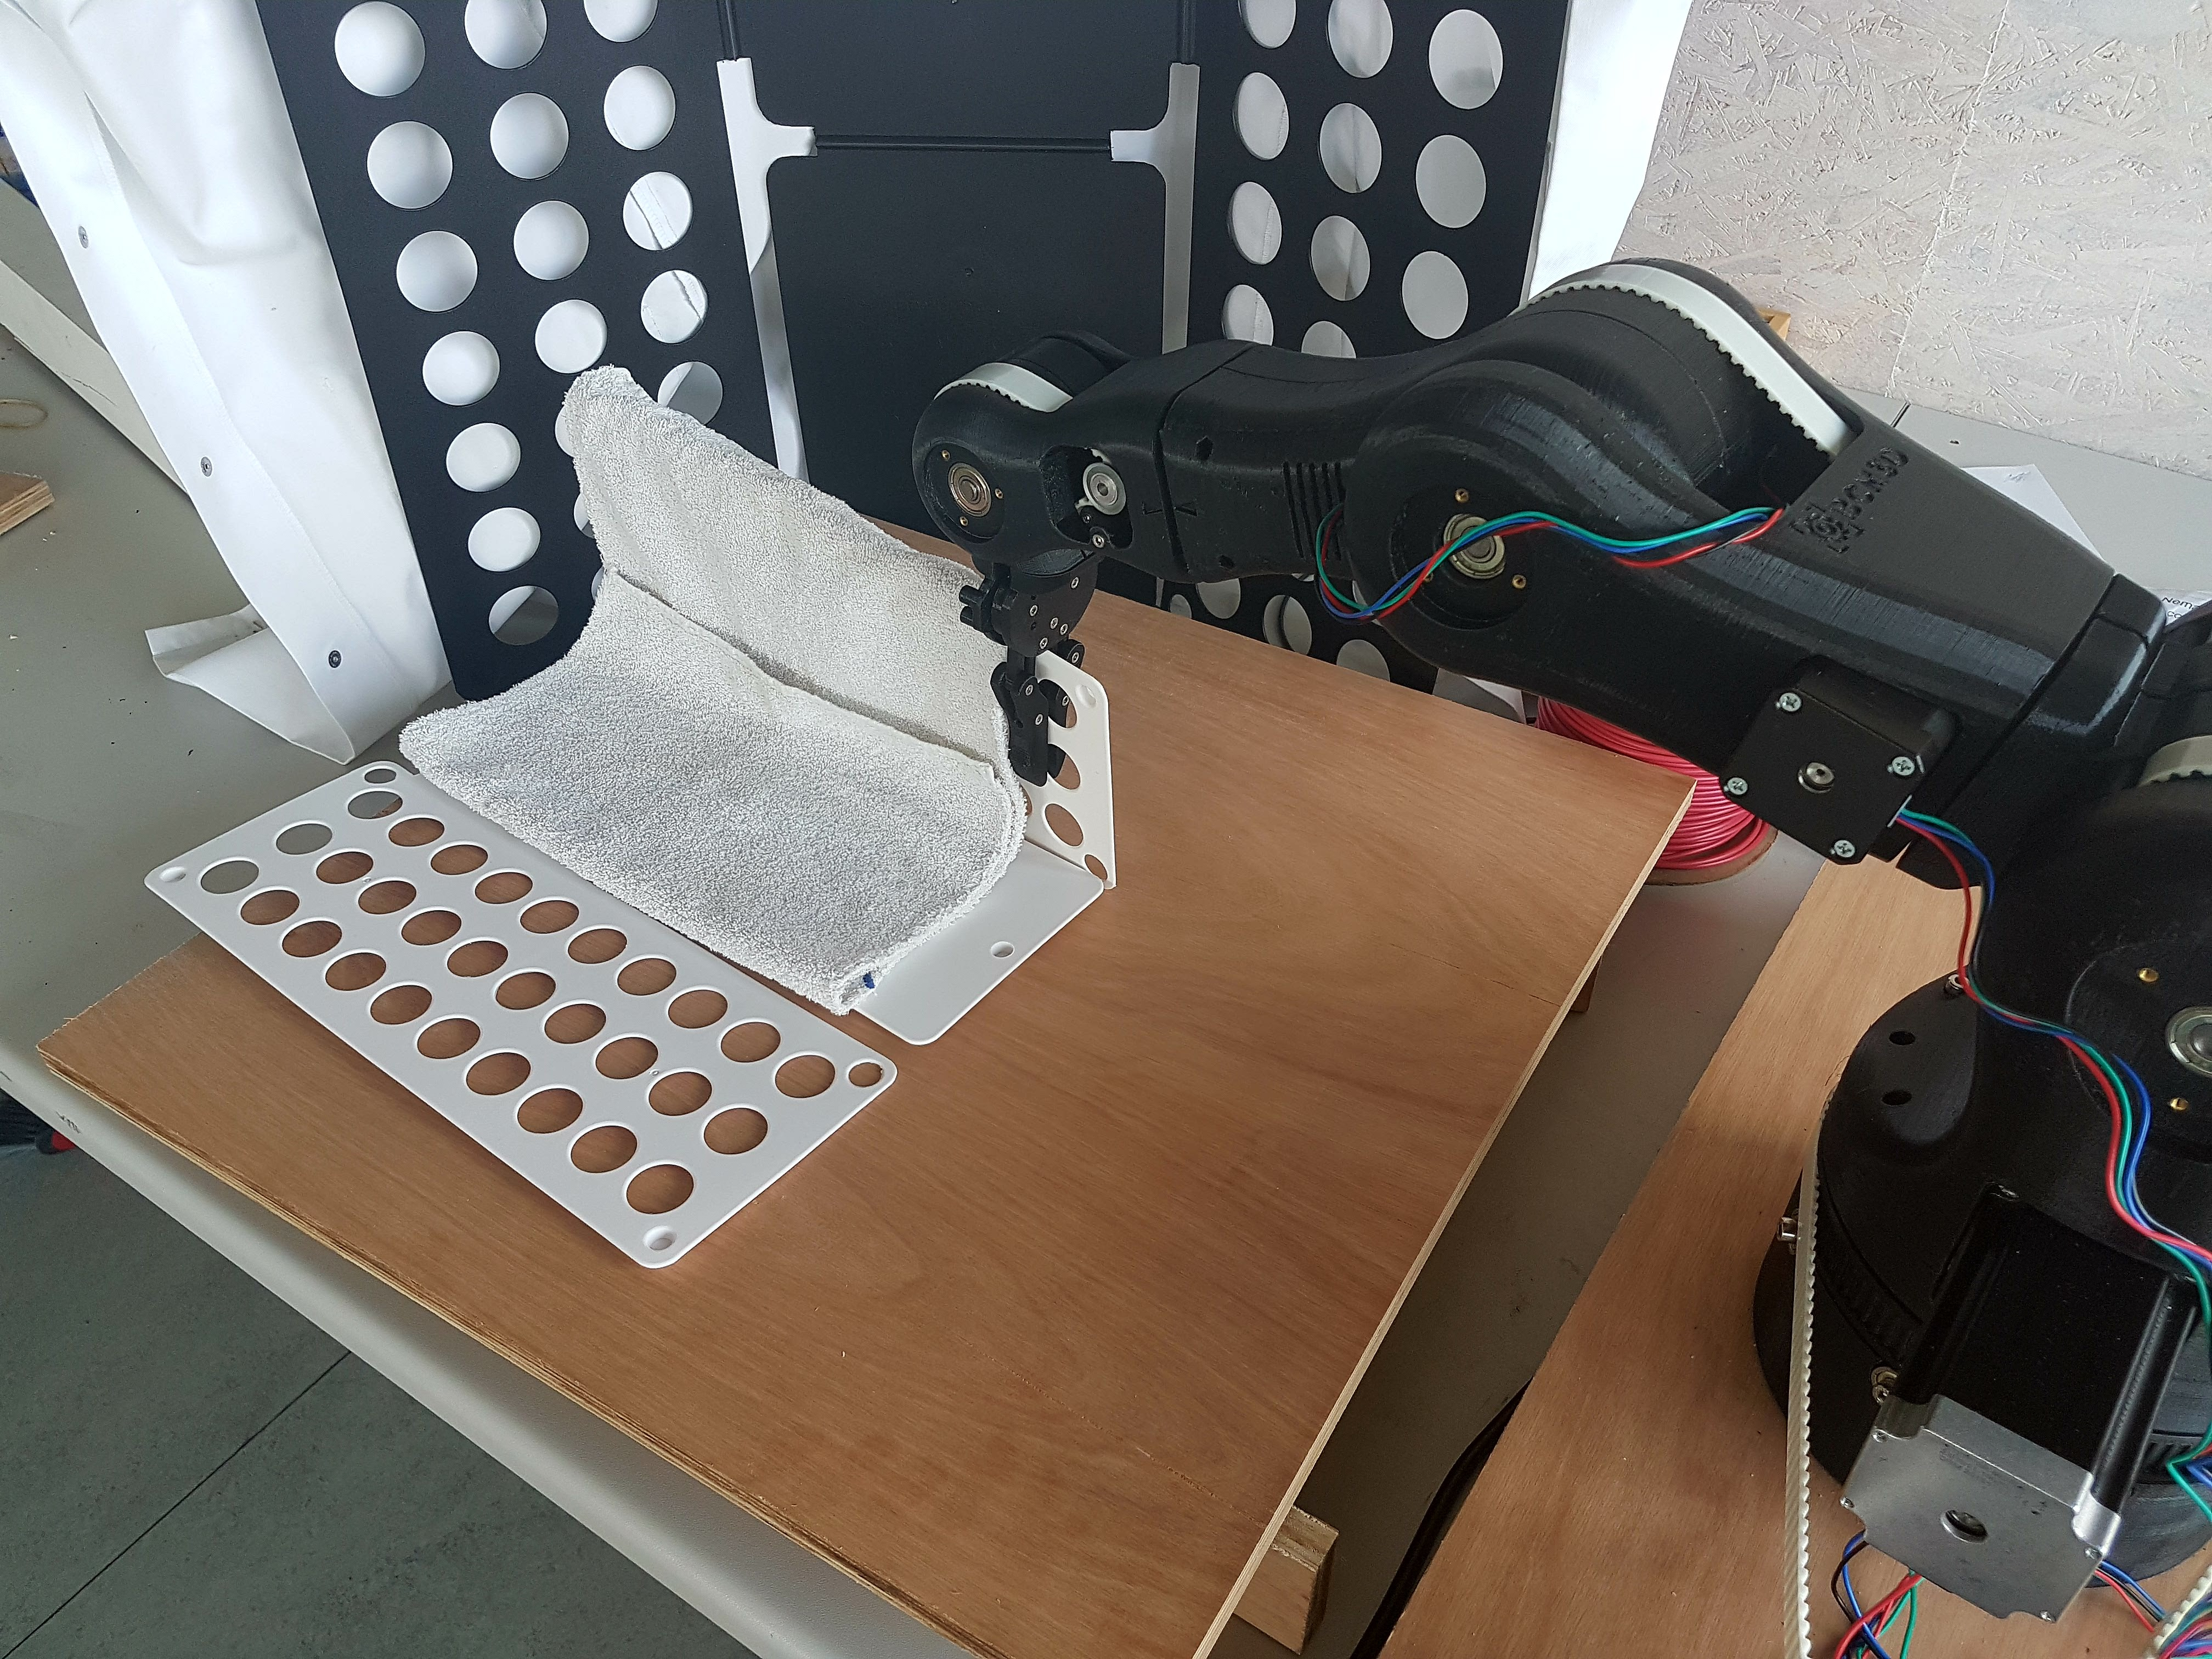
\includegraphics[width=\textwidth]{figures/flipfold_moveo.jpg}
      \label{fig:towards_flipfold}
    \caption{First learning to fold a flip-fold can be considered as an instance of curriculum learning towards learning to fold cloth.}
  \end{figure}
  
The two former approaches of using curriculum learning seemingly indicate an incongruity between manually-specified and fully-learned curricula. In reality, setting the curriculum is a spectrum in which elements of both manual and adaptive specification appear. \textcite{rudin2021learning} for example, learn quadruped locomotion by using a curriculum heuristic that adapts the slope and stairs in the environment based on how far the agent has learned to walk. 
We believe combining heuristic curricula with adaptive and manually-tuned environment elements avoids the instability and premature convergence associated with fully-learned curricula. 
This observation is in fact the overarching theme; we advocate there is a spectrum to be leveraged between programming and data. Finding the balance between engineering and learning parts of the curriculum is an important way forward to accelerate learning, enable Sim2Real transfer and uncover the aspects of the task that makes learning difficult. 

\subsection{Learning from demonstrations}
Other potential gains for accelerating learning can be found by \emph{leveraging demonstration data in RL}. 
Learning from demonstration has a long-standing history in robotics \autocite{Argall2009}. Using demonstrations usually incurs one of the following problems. 
First, learning from demonstration is known to suffer from generalization and exploration issues in the case of behavioural cloning and dataset aggregation respectively \autocite{Ibarz2021}.
Second, it is not always possible to collect a dataset of demonstrations. For example, recent work for combining RL and imitation learning insert kinaesthetically \autocite{vecerik2018leveraging} or teleoperated demonstrations \autocite{Zhu-RSS-18}. However, teleoperating or moving the robot arm manually can be difficult for tasks where dynamics are important like cloth folding or throwing darts. This is why we investigated the use of demonstrations external to the body of the robot in this research. However, using external observations as bootstrap for learning requires solving a correspondence problem between demonstrator and learner. For this reason, we believe that further gains can be found in the avenue of using external demonstrations as self-supervised representation learning method to be used for downstream tasks. We discuss possible technical future work of our method in \cref{sec:conc_future_work}. 

An alternative form of providing demonstrations is in the form of supervision using a scripted policy. Residual RL in particular exploits the spectrum between programming and data by learning a policy that is additively combined with a scripted policy. The residual approach retains a scripted component which allows pushing the agent to the successful and important regions in the state space. When folding clothing, for example, a hand-engineered controller can navigate the agent towards the cloth using simple segmentation methods that were discussed in \cref{ch:sota} of this dissertation. 

\section{Datasets}

Among computational resources and algorithm-centric advances, the availability of large amounts of data was important for deep learning to break through at the turn of the century. Datasets have played a similar role for the success of data-driven methods in robotic manipulation. In the case of learning to grasp objects, Dex-Net \autocite{dexnet2} puts forward a methodology to frame grasping as a supervised learning problem which leads to a qualitative learning signal. Dex-Net relies on generating a massive \emph{dataset in simulation} containing 6.9 million images. This size is approximately 7 times the size of the largest real-life data collection setup of a single institution containing robotic grasping attempts \autocite{Levine2016}. In contrast to rigid object manipulation, there is a dataset scarcity in the domain of cloth folding. The publicly-shared cloth datasets by researchers are primarily vision-based. Augmenting such datasets with tactile sensing is of importance for dealing with occlusions in cloth manipulation. The field could advance forwards with Dex-Net-like datasets containing a data generator containing multiple objects, with different physical properties. A recent, first initiative towards such datasets is executed in \textcite{DefGraspSim} where grasp metrics for volumetric deformables are generated in simulation. Similar implementations for grasping and manipulating cloth could drive the field significantly forward for learning manipulation strategies and understanding cloth dynamics. 

Although synthetic data is easily available with a simulator, it is plagued with transferability problems which makes research for realistic simulations, robust algorithms and system identification crucial. Alternatively, \emph{real datasets} do not suffer from these problems. However, real datasets of cloth folding are rare. Datasets containing multiple modalities of different types of cloths and materials could help learning representations and understanding cloth interactions. Inspiration can be found in the retail fashion that contains high-quality datasets \autocite{DeepFashion, DeepFashion2, FashionAI}. However, the modalities and item interaction are limited making it non-trivial to find possible application avenues for robotic manipulation tasks. A future direction consists of applying the methodology FashionAI \autocite{FashionAI} uses to scale up the data collection and labelling. FashionAI uses experts to disentangle attributes and label a small fraction of the data. Then, they train a network to label the remainder of the dataset. Training is halted when the network makes too many errors which could jeopardize the label quality. Such approach can be used for labelling and understanding human interaction with cloth. 
Real datasets containing example demonstrations of the task, can be used for bootstrapping learning. We filled in this gap with our research by providing a dataset of humans folding clothing (\cref{ch:dataset}). A large-scale dataset with physical robot-cloth manipulations, similar to \autocite{Levine2016} does not exist at time of writing. Ideally, future efforts are directed towards gathering multimodal data of cloth interaction, possibly enriched with large-scale simulated data similar to Dex-Net. This dataset can then be used for understanding material properties of the cloth, bootstrapping learning from the example demonstrations and learning semantic meaningful representations.

Finally, \emph{benchmarking} robotic manipulation is an important step towards progressing the field of object manipulation. Benchmarking manipulation is challenging due to the diverse set of robots, object availability and costly robot interaction time. An additional difficulty is caused by the deformable nature of cloth: the cloth can be initialized in infinite amount of starting configurations which makes it hard to start the task from a common initialization. A significant step towards filling this gap has recently been addressed in the work of \autocite{Camacho2020} and \textcite{garciacamacho2021household} where a standard set of objects, tasks and protocols are introduced for benchmarking common cloth manipulation tasks ranging from folding cloth to partial dressing. Future work can expand on this by including different clothing articles into the object set, considering multiple solution strategies for tasks like folding and extending the task set to cases where multiple objects are in the set. Concerning the evaluation of task performance, the field could use calibrated environments and software tools to measure task performance in a standardized way. Alternatively, our work in \cref{ch:reward_functions} potentially integrates with benchmarks as we provide a methodology to extract a task progression metric. The work of \textcite{Camacho2020} additionally proposes evaluating the performance of the entire system. However, given that the state perception of cloth is of fundamental importance, we find an ImageNet-like dataset for cloth currently missing in the community. This perception cloth dataset should contain multiple types of clothing articles, diverse configurations, interactions and heterogeneous input modalities. 
Ideally, benchmarks and datasets containing real objects are enriched with a simulated counterpart, calibrated on the real data. Given the success of simulation in robotics, researchers could run quick experiments in simulation and transfer results to the real world. 
These benchmarks fundamentally help the field forward as it brings best practices, standardization and comparison of experiments into the complex field of robotic cloth manipulation. 

% Benchmarks toevoegen:
%     Boras - grasp centered analysis 
%     We believe that a proper classification of the types of grasps and manipulation primitives used in handling textile objects is one of the steps necessary to develop a future such benchmark.



\section{Simulation} \label{sec:towards_sim}
Data-driven methods from the machine learning domain have proven extremely powerful for adaptive and robust control. However, they require many examples which are expensive to generate on real, physical systems. The outlook remains that highly parametrized functions such as neural networks will keep on requiring and improving on large amounts of data \autocite{sun2017revisiting}. Hence, simulation remains an important tool for robotic learning to generate large datasets. As distilled in \cref{ch:sota}, there are roughly two roads for exploiting simulations: learning from interaction or constructing large datasets with realistic grasping examples, similar to Dex-Net \autocite{dexnet2}. As of today, it appears the second road, i.e.\ generating datasets, has proven to be commercially exploitable in comparison to learning from interaction. Dex-Net for example, has been commercialized two years after its advent\footnote{https://www.ambirobotics.com/}. Pursuing a similar path for robotic cloth folding is meritful but first requires further research and development in soft body simulators. Specifically,
realistic simulation of friction, material deformation and other physical properties will have to be further developed before the deformable object manipulation domain can follow along the same path as their rigid counterpart. The outlook is promising as  existing and new simulations started supporting soft body simulation, for example MuJoCo 2.0, Isaac\footnote{https://developer.nvidia.com/isaac-gym}, and SoftGym. In addition, state-of-the-art research in cloth simulation recently addressed real-time simulation of realistic cloth and solves inverse control problem like human-assisted dressing and material properties estimation \autocite{Junbang2019,li2021diffcloth}. However, the support for robotics integration is limited. It appears that current robotics researchers have to trade off simulation fidelity and cloth features versus integration possibilities with robotics and control. Hence, future directions should consider a tighter integration between high-fidelity cloth simulation and practicable robot control.

An important characteristic of the cloth simulation is the degree of parallelization. Running many learning environments in parallel has shown to allow learning quadruped locomotion on a single machine within a single day \autocite{rudin2021learning}. We believe this is a strong example that advocates for future cloth simulations to run on GPU in order to run learning environments massively in parallel. Our research addresses this idea with our cloth simulation on \gls{GPU} developed in \cref{ch:simulation}.    

Deformable bodies require reasoning about the shape, dynamics and material properties of the object. This makes neural networks a viable replacement for analytical models in simulations. Neural networks can learn the forward dynamics of cloth from sensory input. Moreover, forward passes through the network can be faster than a forward pass through all simulation sub-steps. 
However, dataset bias is an issue when training machine learning models to predict physics dynamics: world models are trained on a dataset making it is unclear how well they generalize. Complex, learned dynamics models may show visually unrealistic deformations, lose volume over time and cannot deal with occlusion which is bound to happen when manipulating with an end-effector \autocite{Mrowca2018, Li2018}. Therefore, future research efforts should deal with occlusion by incrementally learning the object properties. 
Once again, insights from analytical models of cloth can be exploited in parametrizing the learning model. Graph neural networks, for example, reflect the interconnected particle nature of mass-spring simulation approach to cloth and show promising results for realistic and efficient cloth simulation \autocite{pfaff2021learning}. Alternatively, residual physics uses learned physics on top of an analytical model to predict the error in the forward dynamics \autocite{Golemo2018} or learn fine-grained, unmodelled effects in the simulator from data \autocite{heiden2021neuralsim}.
 
Finally, differentiable simulations allow backpropagating gradients through the physical consequences of actions. Differentiable cloth simulation has been shown to be an effective approach for control problems and estimating material properties \autocite{Junbang2019,li2021diffcloth}.
A future avenue worth exploring is the co-optimization of body and brain: how would the robot morphology evolve if the parametrization of the end-effector is taken into the optimization loop. Outsourcing intelligence from the brain to the body is a principle known as morphological computation \autocite{Rolf2006} and is highly visible in nature. For example, legged animals have their muscles arranged in a way that enables them to use simple neural signals for control \autocite{MacKay-Lyons2002}. 
This principle of outsourcing computation to morphology has been shown to be transferrable to quadruped locomotion by using compliance \autocite{Urbain2021}. The same idea can be used to study how gripper embodiment and control can be co-learned to handle a variety of objects. This research would answer questions about which end-effector designs are optimal for manipulation of cloth and how different material properties lead to different gripper designs. For the application of cloth manipulation, it has already been shown that the choice of gripper design influences the complexity of the task dynamics \autocite{Borras2020}. In order to optimize for such co-design objective, differentiable simulation can be used. By making the simulation and physics differentiable, gradient-based optimization can be used as alternative to evolutionary strategies or \gls{RL}. Gradients provide a direction in which to change the control parameters locally, leading to much quicker convergence \autocite{Degrave2019, li2021diffcloth}.
We prospect that by simultaneous evolving body and brain, new and innovative gripper concepts with competitive grasping performance will arise. 

To summarize, we strongly advocate for further developing the realism and parallelism of cloth simulations that allow for semi-realistic robot-cloth interactions. Ideally, the simulator exposes numerical or analytical gradients which allow gradient-based optimization of inverse problems and robot morphology. Nonetheless, the question remains on how far we can drive the realism of the simulation. A high-quality cloth simulation of Blender, for example, is shown to be not transferrable to the real world in the work of \autocite{Tanaka2018}. Hence, Sim2Real transfer remains an important research direction which we discuss next. 

\section{Sim2Real}
Transferring skills learned in simulation to the real world will remain relevant because further increasing the accuracy of simulators like Bullet and Mujoco(cfr./ \cref{ch:sim}), and making more robust controllers alone will not bridge the Sim2Real gap. In literature, there are a lot of success stories of domain randomization as a method for training robust controller in simulation. However, domain randomization, or more broadly simulation randomization, samples environment parameters uniformly which leads to demanding computational resources. Further research should pinpoint important environment parameters to vary and impose a curriculum for efficient learning. Another useful approach is system identification in which the physical parameters of the simulation is tuned. The discussed differentiable programming approaches for simulation in \cref{sec:towards_sim} merit potential in this regard. 

As a final note, cognitive sciences deem it plausible that humans operate under an intuitive understanding of physics rather than constructing exact physical models of reality \autocite{Baillargeon2011}. This raises the question on how much importance should be dedicated to Sim2Real solutions that focus on tuning the simulation towards the real world as compared to developing models and representations that interpret physics and act on the understanding of these dynamics. We discuss sensing the environment and building representations in the following sections.  

\section{Grippers for robotic folding}
\Textcite{Billard2019} bring to the attention that most robotic applications utilize parallel jaw grippers which are unable to solve tasks that require dexterous manipulation.
Similarly, \textcite{Siciliano2008} note that dexterous, multi-fingered hands have not really been applied to any major application due to reliability, complexity and cost. Recently, \textcite{Borras2020} brought a similar observation to the domain of cloth manipulation that most prior work uses a pinch grasp with both general-purpose and cloth-specific grippers. Indeed, the robot-cloth manipulation community is uncertain about what types of end-effectors are needed for optimally grasping and constraining cloth-like objects. For this purpose, \citeauthor{Borras2020} propose a framework to characterize grasps and manipulation primitives which has given rise to novel gripper designs in \autocite{Donaire2020} for performing cloth-related tasks. 
A next step towards designing beyond anthropomorphic hands requires replacing rigid components with soft elements. Compliant elements lead to easier control and more safety, an aspect important for co-bots and household robots. Soft-bubble \autocite{Naveen2020soft} for example, uses air-filled finger membranes for simultaneous compliant control and tactile sensing.
These developments align with the philosophy that intelligence can be outsourced to the embodiment.
As discussed in \cref{sec:towards_sim}, we can extend these insights and methodologies by co-optimizing embodiment and control. We have argued that simultaneous optimization of body and brain is a research direction containing a lot of potential for optimizing the gripper shape for the robotic cloth manipulation task at hand. Differentiable programming allows computationally efficient co-design of embodiment and control, which will be the ultimate step towards truly effective multifunctional grippers.


% contact grippers with underactuated mechanisms and suction cups could be a promising approach for the manipulation of fresh fruit and vegetables [22]. It is such a gripper that has won the last Amazon Picking Challenge [23]. While pneumatic grippers are useful for grasping, using suction for manipulation if more difficult. Cfr Billard2019 daar over zegt. 

\section{Sensing}

\todo{Eventueel nog een figuur toevoegen met verschillende grippers dat al gemaakt en gebruikt zijn. Idem met instrumented cloth en de sensoren die we al gemaakt hebben. Instrumentatie setup met tekeningen enzo al toevoegen. }

Deep learning has proven to be a strong representation learning method that builds complex concepts out of primitive representations. The bulk of the robotics manipulation research that uses deep learning, leverages vision as input modality for training a deep neural network. While camera images are useful for extracting a global perspective on the shape of the object, capturing small-scale deformations in noisy environments with occlusions and changing lighting conditions is difficult. Moreover, sensing and reasoning about contact forces with the environment remains a problem for data-driven controllers. This is why future research should capitalize on acquiring and fusing multiple modalities. The work of \autocite{lee2020making} paves a way by learning a multi-modal latent space for robotic control tasks. In the deformables domain, tactile information is being used for estimating cloth properties \autocite{yuan2018active}. However, a large barrier to using tactile sensing is the sensor hardware accessibility. \citeauthor{Siciliano2008} note that `tactile sensing always seems years away from widespread utility compared to vision' \autocite{Siciliano2008}. While many types of tactile sensors exist, for example GelSight \autocite{donlon2018gelslim} and FingerVision \autocite{Yamaguchi2017}, it is difficult to create a sensor that is inexpensive, has a fine-grained resolution with high sensitivity and is easy to integrate and use. Nonetheless, research recognizes the need for tactile sensing with cost-effective off-the-shelf sensors like Digit \autocite{digit2020}. In addition, sensors like Soft-bubble \autocite{Alspach2019} where the sensing is intrinsically part of the gripper morphology allow both high contact area grasping and high-resolution sensing. Future robots preferably are equipped with similar soft fingers containing tactile sensing by default. 

Another aspect of tactile sensing is the integration of sensors into the object, a process we labelled \textit{instrumentation} in this dissertation. 
We explored this in \cref{ch:instrumentation} by creating a smart textile embedded with tactile sensing that can communicate the state of the cloth. Future work should focus at increasing the type of forces being measured by embedding pressure, shear, strain and IMU sensors among others. The sensing hardware preferably resembles a sensor \emph{skin} where instrumentation takes place on the surface of the object while minimizing the impact on material properties. This implies that the electronics inside the soft skin should be able to deform to irregular shapes. Inspiration for soft sensor skins can be found in the field of humanoid robots where for example iCub has embedded tactile sensing \autocite{Tomo2018}. Our outlook here is that research in stretchable circuit technology allows further miniaturization for soft skin instrumentation of objects. The soft sensor skin in turn allows using compressed representations for learning downstream tasks on the real platform. 

A missing piece of the instrumentation puzzle is \emph{generalization from instrumented objects to non-instrumented objects}. Similar to the human ability to estimate the outline and texture of an object using touch only, cross-modal prediction models can learn to see by feeling and vice versa. Generally, cross-modal prediction models aim to predict data in one domain from the other. This is an active research domain in the vision and NLP domain in which they aim to generate captions for images, for example \autocite{donahue2015long} among others. In robotics, cross-modal generative models have been used to generate an image based on tactile data and vice versa \autocite{Li2019}. We postulate that similar methods can be used to learn representations that contain invariance to input modality. We elaborate on these ideas, based on our research, in the concluding \cref{ch:conclusion}. 

\section{Representations} \label{sec:towards_sensing_representation}
% DL and NN as representation method
%   Bekijk ook https://journals.sagepub.com/doi/10.1177/0278364918770733?icid=int.sj-full-text.similar-articles.2

In the ideal situation that a rich, high-quality and multimodal dataset can be collected, the question remains on how to generate appropriate representations from it. Our work has demonstrated that useful representations can be learned by using contrasting examples that are mined in a self-supervised manner. Therefore, we support the idea that applying contrastive representation learning methods on cloth datasets described in this chapter leads to rich representations useful for downstream tasks. A remaining question then remains in which part of the cloth manipulation pipeline to insert the representation. Our work has used a smart cloth (\cref{ch:instrumentation}) and cloth folding representation (\cref{ch:reward_function}) in the reward function. An open question remains how to avoid a learning agent exploiting learned reward functions. For this, we draw inspiration from the residual RL and residual physics domain. We hypothesize that \emph{residual reward functions}, an additive reward function of an engineered and data-driven component, could prevent the agent from exploiting the reward function. Alternatively, the learned representation can be used as a state variable. This promising direction is, for example, explored in CURL \autocite{Srinivas2020CURL} where contrastive representations are optimized jointly with the RL objective. 

A final outlook concerns the fundamental question on the appropriateness of deep neural networks in robotics and more specifically, in \gls{RL} that is characterized by incremental learning. Neural networks tend to forget what has been learned when new patterns are acquired. Although replay buffers are used in order to mitigate catastrophic forgetting, approaching neural networks differently on a conceptual level are more promising in our opinion. For example, memory-augmented neural networks represent memory explicitly and train a controller module that learns to store and manipulate memory \autocite{graves2014neural}. An architecture with explicit memory can, for example, learn and retrieve different folding strategies depending on the situation. Furthermore, research should explore beyond connectionist methods. An example is given in the work of \textcite{Jia2019} who demonstrate that tree-based methods can still be competitive in an era dominated by deep learning. Their work considers cloth manipulation tasks by exploiting the non-parametric nature of random forests to dynamically change the number of leaf nodes based on the given imitation data and new cloth configurations.


\section{Future outlook on the field of robotic cloth manipulation} % TODO: andere titel. Bv future outlooks on cloth folding

The field of robotic manipulation of clothing items has evolved from highly engineered pipelines to data-driven methods the past decade. The impressive results of \gls{RL} prompted the community to shift from one end of the spectrum, i.e.\ fully decomposed sub-systems, to the other end, i.e.\ end-to-end pipelines. Recent trends show that researchers discovered the limitations of end-to-end \gls{RL} and are now finding the centrum of this spectrum. 
This centrum involves renewing the attention for \emph{hardware} \todo{Democratizering van hardware: accessibility van hardware: prijs, open source,
en toon ook maar dat wij doen: wij hebben onze setup en data beschikbaar gemaakt. 
}, which has recently been addressed with a framework for understanding the links between grasp types and gripper for cloth. A major insight that helps in this regard is outsourcing intelligence to the hardware embodiment for robust control. By \emph{co-optimizing the body and brain}, the chain is closed and task-effective gripper designs with integrated control arise. 
Using \emph{soft materials and integrated sensing} will play a vital role in fabrication of grippers as clothing items have notoriously difficult state estimation.
To facilitate state estimation, we foresee an important role for \emph{instrumentation} towards smart cloth using robot sensing skin from stretchable circuit technology. 
We hypothesize that the resulting gripper and smart cloth implementations should be used for the \emph{generation of a multimodal dataset} and benchmarks containing cloth-robot interactions. Ideally, such datasets contain a virtual counterpart calibrated on the real data. However, we believe that simulations should not pursue \qty{100}{\percent} realism. Rather, the community should focus on developing models and representations that help understanding and acting on physics in order to reduce the Sim2Real gap. 
The multi-modalities of the simulated and real data can be used to \emph{learn meaningful representations} of deformations for downstream tasks.
These tasks can be factorized at a level that interactions among sub-problems are small and most of the complexity is handled by the sub-systems. % Let op: de vraag hier gaat zijn op welk niveau de factorizatie zich afspeelt. Dit is een open vraag. 
Finding solutions for the tasks contained in the sub-systems requires striking a balance between programming and leveraging data. A central philosophy we deem important is the presence of a \emph{residual} component that merges prior knowledge of analytical models with the data-driven components of morphology, simulation, imposed curriculum, reward signals and finally, control policies. 
 
Ik mis nog iets over self-supervised learning and curriculum hierin, twee dingen waar ik sterk in geloof.  

Er ontbreekt hier een generaltiy claim: terug open trekken. Hele robotica community aspect, benchmarks, citizen science, opensourcing, reproduceerbaarheid, democratizering van hardware;alles mag hier herhaald worden. Schrijf eerst al deze aspecten bulletgewijs uit en vat het dan samen in een generality claim zin. 
zeker omdat je hier een open source dataset hebt, hardware ontwikkelt hebt.  

% Finally, self-supervision is a tool to generate a lot of inexpensive data. 

% The dream:

% PREREQUISITES
%  THE DATA 
    %  a dataset of diverse clothing items with multiple modalities. Interactions on these items. Have a simulated part that is calibrated to the real object their properties. This simulation interfaces with common robotics tools and runs in parallel. There is a natural curriculum heuristic included for efficient learning. 
% THE HARDWARE
    % The required hardware is based on the work of \autocite{Borras2020} or co-evolved with the controller. 
    % Sensing is included
% I would use this dataset for learning a useful representation based on self-supervised method proposed in this research. 

\end{document}